\section{实验与结果分析}
本章将对\ref{sec:chapter03}中所设计的GNSS位置欺骗攻击检测算法进行实验,展示相关的数据细节(训练数据与实验所用数据集)以及实验结果。
\subsection{数据集概述与实验结果分析}
本文中用于训练模型以及测试算法所使用到的数据集是来自Comma.ai的Comma2k19数据集\cite{commaai}。该数据集中包含从加州圣何塞到旧金山共2019段行程记录,每段时长1min。数据集中包含前置摄像头、GPS、温度计以及一个九轴IMU等传感器的数据,以及行驶过程中车内CAN的所有数据。数据采集过程中,Comma.ai使用u-blox M8 GNSS模块采集数据,其水平位置进度为2.5m;此外,Comma.ai还使用了一个开源GNSS数据处理库Laika来进一步降低定位误差,并最终使定位误差下降了40\%。
训练检测模型需要用到车辆的速度、转向角以及前向加速度作为输入。速度与转向角数据可以从CAN中获得,而前向加速度则可以从IMU中获得。另一方面,训练过程中,还需要用到车辆在相邻时间戳之间的行驶距离。这可以通过GNSS数据计算得到。需要注意的是,由于地球并非平面,因此在计算距离的时候,不能直接使用欧式距离计算公式,而应该使用哈弗森大圆公式计算。如公式\ref{eq:Haversine}所示。
\begin{equation}
    d=2r\sin^{-1}\sqrt{\sin^2\frac{\varphi_2-\varphi_1}{2}+\cos(\varphi_1)\cos(\varphi_2)\sin^2\frac{\psi_2-\psi_1}{2}}
    \label{eq:Haversine}
\end{equation}
其中,$d$表示地球表面两点之间的距离,$r$是地球半径;$\varphi_1$,$\varphi_2$表示当前位置的弧度制纬度,$\psi_1$,$\psi_2$表示下一相邻时刻位置的弧度制经度。
以上数据在本文中用于训练GNSS欺骗检测模型,同时在用于测试算法效果。其中,训练集包含14399项数据(每一项包括速度、转向角、前向加速度、与上一时间戳的距离以及时间戳);测试集中则包含共11998项数据。需要说明的是,由于数据集中并没有包含受欺骗的GNSS数据,因此,需要在原数据的基础上进行改动,才能得到欺骗数据。本文主要通过软件QGIS,在原始数据的Southbay Fwy路段上,从第一个是什么个数据项开始,加入有攻击意义的偏移,从而生成可用的测试数据。原数据与加入偏移后的测试数据如图\ref{fig:map}所示。其中,黑色线条表示真实轨迹,红色线条表示欺骗数据轨迹。
\begin{figure}
    \begin{center}
        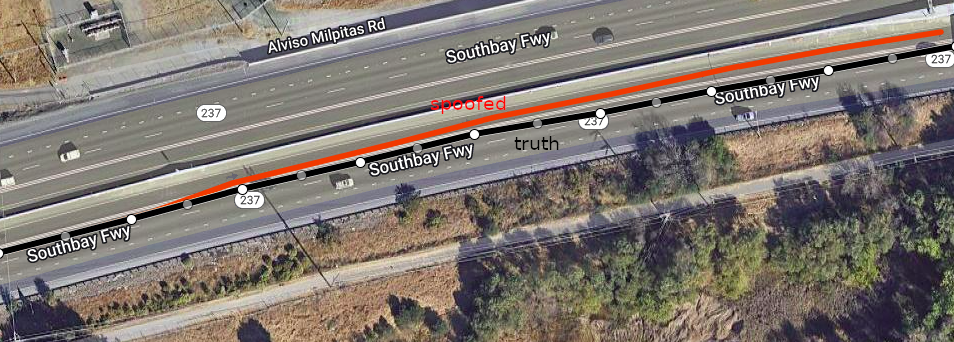
\includegraphics[width=0.95\textwidth]{Map_with_caption.png}
    \end{center}
    \caption{原数据与欺骗数据在地图上的轨迹对比}
    \label{fig:map}
\end{figure}
实验表明,当第1932个数据项被输入到模型时,模型检测到欺骗发生。这说明算法可以有效检测到异常的GNSS定位数据。
\subsection{本章小结}
本章主要对模型训练以及算法测试所用到的comma2k19数据集做了简要介绍,同时阐述了如何利用哈弗森大圆公式从原数据中提取出真正需要的数据。另外,本章还展示了基于comma2k19所进行的验证实验的实验结果。实验表明,本文所设计的GNSS位置欺骗攻击检测算法可以有效检测到受欺骗的异常GNSS数据。
